\documentclass[oneside, paper=A4, DIV=15]{scrartcl}
\documentclass[oneside, paper=A4, DIV=15]{scrartcl}
\usepackage[english]{babel}
\usepackage[utf8]{inputenc}

% Font settings
\usepackage{libertine}
\usepackage{libertinust1math}
\usepackage[T1]{fontenc}

% Math, symbols, units
\usepackage{siunitx}  

% Typography
\usepackage[auto]{microtype}

% Author information
\usepackage{authblk}
\renewcommand\Authand{, }
\renewcommand\Authands{, }

% Bibliography
\usepackage[style=authoryear, maxnames=2, minnames=1, sorting=nyt, backend=biber]{biblatex}
\addbibresource{references.bib}
\bibliography{references}
\nocite{*} 

% PDF settings
\usepackage[
pdftitle={},
pdfsubject={},
pdfauthor={},
pdfkeywords={},  
hidelinks
]{hyperref}

\usepackage{graphicx}
\usepackage{amsmath} 
\usepackage{verbatim}   
\usepackage{tabularx,booktabs}
\usepackage{array}    
\usepackage{pgfgantt}


\subject{Exposé Bachelor's Thesis}
\title{Detecting Gender Bias in English-German Translations Using NLP}
\author{Khanh Linh Pham, 77211916753}
\affil{Supervisor: Prof. Dr. Diana Hristova}
\affil{Hochschule für Wirtschaft und Recht Berlin}
\date{\today}

\begin{document}

\maketitle

\section{Motivation}
With the growing availability of free Machine Translation (MT) tools capable of handling complex sentences, ensuring the accuracy and fairness of these translations becomes increasingly significant. However, when translating between languages with and without grammatical gender, there is a risk of incorrect gender assignment. For example, the English sentence "The surgeon is hard-working" is translated into German as "Der Chirurg ist fleißig" using Google Translate and DeepL. This assigns a male gender instead of remaining neutral or offering both masculine and feminine options. Unbeknown to the tool user, such biased translations can amplify discrimination and inequality \parencite{braccini_does_2024}, given the widespread use of MT in both public and business contexts. Thus, this thesis aims to explore gender bias in English-German MT by developing a binary classification model based on Natural Language Processing (NLP). The goal is to help users identify potential bias in translations, raising awareness and promoting the creation of fairer AI systems.


Recent years have seen extensive research on bias in MT. A systematic review of the literature by \textcite{shrestha_exploring_2022} offers a thorough overview of this issue, detailing its scope, impact, and key findings relevant to my thesis. Several case studies comparing English to both grammatical-gender languages (e.g., Spanish, Italian) and non-gender-marking languages (e.g., Hungarian) consistently identify biases, including the assignment of stereotypical gender roles and a default tendency to use male pronouns \parencite{stanovsky_evaluating_2019, prates_assessing_2019, braccini_does_2024}. The methodologies used in these studies will be valuable for my own implementation. Lastly, the study by \textcite{lardelli_building_2024} on the challenges of translating English into German lays the foundation for my analysis. It provides data for testing the translation of gender-neutral terms in context, as well as a gender-fair German dictionary, both of which I can build upon.


\section{Research Question}

To address this issue, the following research question will be investigated:
\begin{quote}
    \textit{How can a NLP-based binary classification model detect gender bias in English-German translations?}
\end{quote}


\noindent This question can be broken down into four sub questions, each depicting a milestone of the research: \textbf{(1)} Literature review, \textbf{(2)} Data collection and preprocessing, \textbf{(3)} Implementation and \textbf{(4)} Benchmarking and discussion of results.


\section{Methodology}
\begin{description}

\item[(1) Literature Review:] 
This thesis places a focus on the practical implementation. The primary aim is to develop a system for detecting gender bias in English-German translations. As such, the literature review does not aim to provide a comprehensive theoretical analysis. Its role is instead limited to establishing the conceptual and technical context for the implementation. An overview of how the literature is used and how sources were selected is provided in table \ref{tab:overview_literature}.

Since Machine Learning (ML) is a rapidly evolving field and older studies may be outdated, only publications from 2015 onward are considered. Additionally, only publicly available English sources are included. Literature was primarily found using keyword-based searches on Google Scholar. Initial search terms such as "gender bias" and "machine translation" yielded over 18,000 results. Abstract screening and citation analysis helped narrow the scope to a few foundational works, including \textcite{prates_assessing_2019}, \textcite{stanovsky_evaluating_2019}, and \textcite{cho_measuring_2019}. These studies clearly demonstrate the presence of gender bias in MT systems and its relevance in the ML context. They were chosen because they do not focus heavily on technical implementation but instead highlight the differences between gendered and non-gendered languages. Case study results are presented in a clear, accessible way, making them a solid foundation to build upon in this thesis.

From these core papers, both backward and forward citation searches were used to expand the literature base. The backward search often led to older, more conceptual texts, which help define the relevance of the topic overall. In contrast, forward citation search surfaced more applied work, including case studies on specific language pairs. For the forward search, the results were refined using more specific keywords such as “gender bias in English-German machine translation” and “occupational bias in translation”. To cover the technical side, terms like “AI” and “ML” were added. One key resource found through this process is \textcite{shrestha_exploring_2022}, which provides a structured overview of current research on gender bias in MT. It helps define the current state of the field and its limitations without requiring deeper engagement in literature theory. Overall, the targeted search approach revealed a clear research gap: while the existence of bias in MT is well-documented, open-source tools addressing this problem, particularly for English-German translation, are limited. Studies focusing on this language pair generally remain rare.

After establishing that bias exists, the search shifted to sources discussing its real-world consequences. These studies quantify the impact of biased translations, especially in gendered languages like German. For example, \textcite{savoldi_what_2024} and \textcite{bolukbasi_man_2016} discuss how bias in MT can reinforce stereotypes or increase correction costs in post-processing.

To inform the technical design, the search was extended using \href{https://www.perplexity.ai/}{Perplexity.ai}. This tool supports precise prompting and is especially useful for identifying datasets, translation models, and technical papers. Prompts such as “Find datasets for training and testing a gender bias detection system for English-German translations” or “What are lightweight, open-source English-German translation models for Python?” were used. Once specific tools or models were identified, their documentation and supporting literature were manually reviewed.

So far, 17 papers have been collected to support the thesis. They cover key concepts, technical methods, and tools related to gender bias in English-German translation. This selection will be adjusted as the research develops and specific requirements become clearer. The full list of references can be found in section \ref{sec:References}.

\begin{table}[h!]
\centering
\renewcommand{\arraystretch}{1.3}
\begin{tabularx}{\textwidth}{|X|X|X|}
\hline
\textbf{Purpose} & \textbf{Method of Finding} & \textbf{Preliminary Sources} \\
\hline
Define core concept of gender bias in MT & Keyword-based search & \textcite{prates_assessing_2019}, \textcite{stanovsky_evaluating_2019}, \textcite{cho_measuring_2019}, \textcite{shrestha_exploring_2022} \\
\hline
Establish relevance of the topic & Backward citation search & \textcite{bolukbasi_man_2016}, \textcite{savoldi_what_2024}, \textcite{godsil_effects_2016}, \textcite{braccini_does_2024} \\
\hline
Justify technical design decisions & Focused search via Perplexity.ai + manual search & \textcite{devlin_bert_2019}, \textcite{lardelli_building_2024}, \textcite{tiedemann_opus-mt_2020}, \textcite{stella_dataset_2021}, \textcite{savoldi_mgente_2025}, \textcite{papineni_bleu_2001} \\
\hline
Identify research gap & Forward citation search & \textcite{lardelli_building_2024}, \textcite{gete_does_2024}, \textcite{kappl_are_2025}, \textcite{unior_nlp_research_group_university_of_naples__gender_2023} \\
\hline
\end{tabularx}
\caption{Overview of literature use and discovery methods}
\label{tab:overview_literature}
\end{table}

    
\item[(2) Data Collection and Preprocessing:] 

As mentioned in (1), I have collected relevant datasets from existing research. The preliminary list is shown in the table below, alongside short descriptions and content summaries.

\begin{table}[h!]
    \centering
    \renewcommand{\arraystretch}{1.3}
    \begin{tabularx}{\textwidth}{|X|X|X|}
    \hline
    \textbf{Dataset} & \textbf{Description} & \textbf{Content} \\ \hline
    \href{https://huggingface.co/datasets/FBK-MT/mGeNTE}{mGeNTE en-de} \parencite{savoldi_mgente_2025} & Multilingual Gender-neutral Translation Evaluation dataset used to assess gender bias in MT systems. & \textasciitilde1,500 English sentences with gender-neutral and gendered . \\ \hline
    \href{https://github.com/g8a9/building-bridges-gender-fair-german-mt}{Building Bridges Dictionary} \parencite{lardelli_building_2024} & Curated bilingual dictionary for promoting gender-fair language in English-German MT. & \textasciitilde1,000 German gender-neutral and gender-inclusive sentences and their English translations.  \\ \hline
    \href{https://research.google/blog/a-dataset-for-studying-gender-bias-in-translation/}{Translated Wikipedia Biographies} \parencite{stella_dataset_2021} & Dataset of English Wikipedia biographies automatically translated into multiple languages, used to test gender bias in MT outputs. & \textasciitilde1,500 translated biography sentences. \\ \hline
    \end{tabularx}
    \caption{Overview of Selected Datasets}
    \label{tab:datasets}
\end{table}

Data preprocessing aims to ensure the quality and fairness of the data.
The bias labels and translations of the chosen datasets will be validated first. This requires checking that each example has the bias labels applied correctly and that the translations are accurate. Validation will be done through a mix of manual checks and automated checks using language models and translation systems. The dataset will then be checked for balance to make sure that gender-related terms and categories are not significantly over- or under-represented to avoid adding bias to the model. If necessary, under-represented categories will be added as needed, and over-represented categories will be decreased.

Ultimately, the goal is to combine the validated data from all datasets. The merged dataset should have at least 6,000 entries to support a proper binary classification task \parencite{pecher_comparing_2024}. This dataset will be used to fine-tune the classification model explained in (3). Each data point will contain:

\begin{itemize}
    \item English sentence "eng\_source\_sentence"
    \item German translation "ger\_translation"
    \item Source Gender "source\_gender" (male/female/neutral)
    \item Translation Gender "translation\_gender" (male/female/neutral)
    \item Bias label "bias\_label" (1 for biased, 0 for unbiased)
\end{itemize}


\item[(3) Implementation:]

The focus of this thesis will be on \textbf{Fine-tuning a Pre-trained BERT Model to Detect Gender Bias in English-German Translations}. The demo will allow the user to input an English sentence, which is translated into German. If a bias is detected, the translation will be flagged. 

The model will analyze translated text for the following labeling rules:

\begin{table}[h]
\centering
\begin{tabular}{llc l}
\toprule
\textbf{Source Gender} & \textbf{Translation Gender} & \textbf{Label} & \textbf{Example} \\
\midrule
male or female & matches source gender & 0 & "She is a doctor" $\rightarrow$ "Sie ist Ärztin" \\
male or female & neutral & 1 & "She is a doctor" $\rightarrow$ "Arzt" \\
male or female & opposite gender & 1 & "She is a doctor" $\rightarrow$ "Er ist Arzt" \\
neutral & neutral & 0 & "The teacher" $\rightarrow$ "Lehrkraft" \\
neutral & gendered (male or female) & 1 & "The teacher" $\rightarrow$ "Lehrer" \\
\bottomrule
\end{tabular}
\caption{Bias labeling rules based on source and translation gender}
\label{tab:bias_labeling_rules}
\end{table}

Fine-tuning a pre-trained multilingual BERT model was chosen over training a model from scratch due to constraints on computational resources and time. Fine-tuning enables the adaptation of a pre-trained model to a specific task, in this case, binary classification of gender bias. Since BERT has been trained on a large, multilingual corpus, it is well-suited to capture complex language patterns. This approach not only enhances performance but also accelerates training, especially when data is limited \parencite{devlin_bert_2019}. This approach improves performance and speeds up training compared to starting from scratch, especially when data availability is limited.

The implementation will be carried out in the steps outlined below:

\begin{enumerate}
    \item \textbf{Dataset Preprocessing}
    \begin{itemize}
        \item \textbf{Purpose:} Prepare the merged dataset for input into the BERT model. 
        \item \textbf{Details:} Combine the English source sentence and German translation, separating them with the [SEP] token.
        \item \textbf{Example:} "She is a doctor. [SEP] Sie ist Ärztin."
    \end{itemize}
    
    \item \textbf{Tokenization}
    \begin{itemize}
        \item \textbf{Purpose:} Tokenize the sentences, converting them into token IDs compatible with BERT.
        \item \textbf{Details:} Use BERT’s multilingual tokenizer to split the sentences into subword tokens.
        \item \textbf{Tool:} BertTokenizer.from\_pretrained("bert-base-multilingual-cased")
    \end{itemize}

    \item \textbf{Model Building}
    \begin{itemize}
        \item \textbf{Purpose:} Use BERT for sequence classification with a binary classification head.
        \item \textbf{Details:} Use "BertForSequenceClassification" to build the model. This adds a layer for classification on top of the pre-trained BERT model.
        \item \textbf{Tool:} BertForSequenceClassification.from\_pretrained("bert-base-multilingual-cased",  num\_labels=2)
    \end{itemize}
    
    \item \textbf{Model Training}
    \begin{itemize}
        \item \textbf{Purpose:} Fine-tune BERT on the dataset to classify translations.
        \item \textbf{Details:} Train the model using backpropagation and a cross-entropy loss function to minimize classification errors.
        \item \textbf{Tool:} Hugging Face's Trainer API.
        \item \textbf{Optional Hyperparameter Tuning:} Experiment with learning rate, batch size, and number of epochs to optimize validation performance.
    \end{itemize}

    \item \textbf{Model Evaluation}
    \begin{itemize}
        \item \textbf{Purpose:} Evaluate the trained model to assess its classification performance.
        \item \textbf{Details:} Use standard metrics such as accuracy, precision, recall, and F1-score.
        \item \textbf{Tool:} Hugging Face's Trainer API's Trainer.evaluate().
    \end{itemize}
    
    \item \textbf{Model Saving and Inference}
    \begin{itemize}
        \item \textbf{Purpose:} Persist the fine-tuned model and set up an inference pipeline for new inputs.
        \item \textbf{Details:}  
        Saving the model ensures reproducibility and avoids expensive re-training.  
        An inference pipeline allows the demo to load the model, tokenize new sentence pairs and predict bias.
    \end{itemize}
\end{enumerate}


The technology stack includes \textbf{Python} for the backend and \textbf{Streamlit} for the web demo. I will build the application locally. Figure \ref{fig:demo_image}, which was created using Streamlit, illustrates what the User Interface could look like, though it does not include the bias flagging feature yet.


For the translation model, I will use \textbf{\href{https://github.com/Helsinki-NLP/Opus-MT?tab=readme-ov-file}{Opus-MT}}. I considered two criteria in my choice: 1) Open-source availability and 2) Lightweight design for optimizing performance. While Opus-MT will be the primary translation model, I may consider adding more models or even Large Language Models (LLMs) that fit my two criteria if it is feasible within the scope of the project. Additionally, as an optional add-on, I might include a justification for the gender flag. This would better explain the reason for the flag to the user and increase the usability of the tool.

\begin{figure}[htbp]
    \centering
    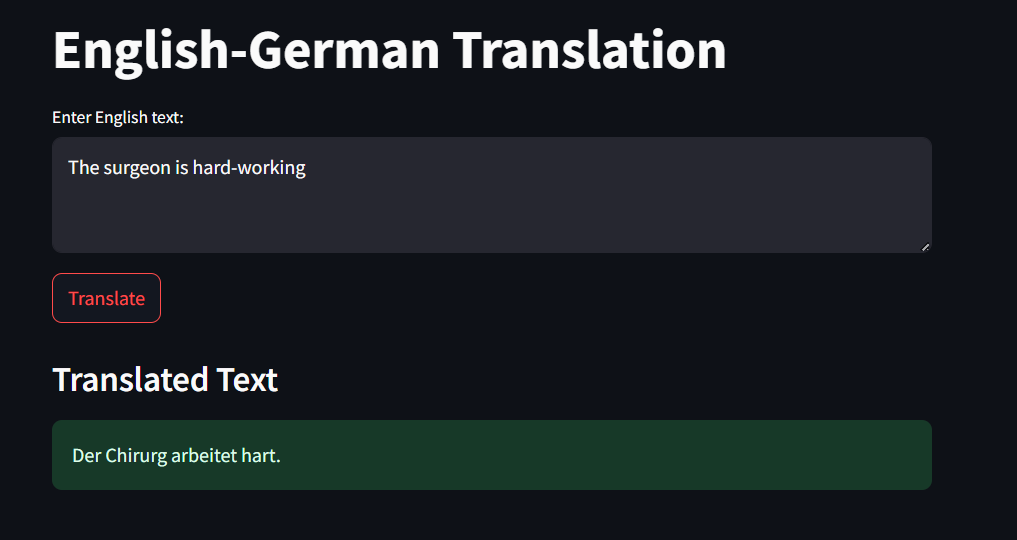
\includegraphics[width=0.8\textwidth]{images/Screenshot_Frontend.png}
    \caption{Frontend Example}
    \label{fig:demo_image}
\end{figure}

\item[(4) Benchmarking and Discussion of Results:] 

After implementing the model, I plan to manually evaluate it by inputting various sentences and different types of bias to assess its performance. This includes the analysis of any errors to gain a deeper understanding of the model's behavior and limitations. I will highlight notable examples of both errors and successes to provide valuable insights into its strengths and weaknesses. The performance results will then be visualized using graphs. 

This process also offers an opportunity to refine the implementation in order to make adjustments where needed. Moreover, I will compare my evaluation outcomes with the claims made in the analyzed literature, determining whether they confirm or challenge existing findings.

Finally, I will address the limitations of my work, outline potential improvements, and suggest what could be added to enhance the model's performance and applicability.


\end{description}


\section{Expected results}
\begin{description}

\item[(1) Literature Review:]
Summary of recent research on gender bias in MT (esp. English-German); identification of key bias types (e.g., male defaults, stereotypes); foundational explanations of NLP concepts and translation systems; research gap: lack of lightweight, explainable detection tools.

\item[(2) Data Collection and Preprocessing:]
Cleaned, balanced dataset with bias labels, stored in one CSV for reproducibility; Python code for validation and preprocessing; insights on bias distribution across datasets.

\item[(3) Implementation:]
Working classification model that detects gender bias in translations with a target accuracy of at least 85\%; Streamlit demo with user input, bias flagging, and optional explanations.

\item[(4) Benchmarking and Discussion of Results:]
Performance metrics (accuracy, precision, recall); example successes and failures; comparison with findings from literature; discussion of limitations and future improvements.

\end{description} 

\section{Expected Outline}
\begin{enumerate}
  \item \textbf{Introduction}
    \begin{itemize}
      \item Motivation
      \item Research Question and Objectives
    \end{itemize}

  \item \textbf{Theoretical Foundations}
    \begin{itemize}
      \item Terminology and Definitions
      \item Social Implications of Gender Bias in Language
      \item State of Research
    \end{itemize}

  \item \textbf{Methodology}
    \begin{itemize}
      \item Research Design
      \item Implementation Overview
    \end{itemize}

  \item \textbf{Data Collection and Processing}
    \begin{itemize}
      \item Dataset Selection
      \item Preprocessing Steps
      \item Data Limitations and Challenges
    \end{itemize}

  \item \textbf{System Implementation}
    \begin{itemize}
      \item Tool Architecture and Workflow
      \item Integration of Translation and Bias Detection
      \item UI
    \end{itemize}

  \item \textbf{Results and Evaluation}

  \item \textbf{Discussion}
    \begin{itemize}
      \item Interpretation of Results
      \item Comparison with Existing Work
    \end{itemize}

  \item \textbf{Conclusion}

  \item \textbf{Limitations and Future Work}
    \begin{itemize}
      \item Methodological Limitations
      \item Suggestions for Further Research
    \end{itemize}
\end{enumerate}


\section{Expected Timeline}
% !TEX root = expose.tex
\begin{ganttchart}[
    vgrid, hgrid, 
    x unit=1cm,
    y unit title=0.75cm,
    y unit chart=0.5cm,
    title height=1,
    milestone left shift=.1,
    milestone right shift=-.1,
    % Appearance of Groups
    group left shift=0,
    group right shift=0,
    group peaks tip position=0,
    group peaks height=0.2,
    %
    title label font=\small,
    bar label font=\small,
    group label font=\small\bfseries,
    milestone label font=\small\itshape,
    ]{1}{12}
    % Total Time in Weeks
    \gantttitle[]{Total Time in Weeks}{12} \\
    \gantttitlelist{1,...,12}{1} \\

    % Research and Foundations
    \ganttgroup{Research and Foundations}{1}{2} \\
    \ganttbar{Literature Review}{1}{1} \\
    \ganttbar{Learn NLP + Tools}{2}{2} \\
    %
    \ganttmilestone{Research and Foundations Complete}{2} \\

    % Methodology + Data
    \ganttgroup{Methodology + Data}{3}{4} \\
    \ganttbar{Define Method}{3}{3} \\
    \ganttbar{Select and Preprocess Data}{4}{4} \\
    %
    \ganttmilestone{Methodology and Data Complete}{4} \\

    % Implementation I
    \ganttgroup{Implementation I}{5}{6} \\
    \ganttbar{OpusMT Setup}{5}{5} \\
    \ganttbar{Gender Bias Detection Prototype}{6}{6} \\
    %
    \ganttmilestone{Implementation I Complete}{6} \\

    % Implementation II + Results
    \ganttgroup{Implementation II + Results}{7}{8} \\
    \ganttbar{Refine Implementation}{7}{7} \\
    \ganttbar{Run Evaluation}{8}{8} \\
    %
    \ganttmilestone{Implementation II Complete}{8} \\

    % Analysis + Discussion
    \ganttgroup{Analysis + Discussion}{9}{10} \\
    \ganttbar{Analyze Results}{9}{9} \\
    \ganttbar{Write Discussion}{10}{10} \\
    %
    \ganttmilestone{Analysis and Discussion Complete}{10} \\

    % Final Writing + Edits
    \ganttgroup{Final Writing + Edits}{11}{12} \\
    \ganttbar{Write Conclusion and Final Sections}{11}{11} \\
    \ganttbar{Proofreading + Submission}{12}{12} \\
    %
    \ganttmilestone{Thesis Complete}{12}
\end{ganttchart}




 
\section{References}\label{sec:References}
This is an initial selection of works relevant to the thesis and will be updated as research develops.
\printbibliography[heading=none]

\begin{center}
\end{center}


\end{document}
